%% LyX 2.1.4 created this file.  For more info, see http://www.lyx.org/.
%% Do not edit unless you really know what you are doing.
\documentclass[ruled]{article}
\usepackage{courier}
\usepackage[latin9]{inputenc}
\usepackage[letterpaper]{geometry}
\geometry{verbose}
\usepackage{algorithm2e}
\usepackage{amsmath}
\usepackage{graphicx}
\usepackage{esint}
\usepackage[unicode=true,
 bookmarks=false,
 breaklinks=false,pdfborder={0 0 1},backref=section,colorlinks=false]
 {hyperref}

\makeatletter

%%%%%%%%%%%%%%%%%%%%%%%%%%%%%% LyX specific LaTeX commands.
\providecommand{\LyX}{\texorpdfstring%
  {L\kern-.1667em\lower.25em\hbox{Y}\kern-.125emX\@}
  {LyX}}

%%%%%%%%%%%%%%%%%%%%%%%%%%%%%% User specified LaTeX commands.
\title{DS-GA 1003: Machine Learning and Computational Statistics\\
Homework 7: Bayesian Modeling} 
\date{} 

\usepackage{amsfonts}\usepackage{capt-of}
%\usepackage{url}
\usepackage{graphicx}
\usepackage{color}
\usepackage{bbm}
\usepackage{enumerate}
\newcommand{\carlos}[1]{\textcolor{red}{Carlos: #1}}
\newcommand{\field}[1]{\mathbb{#1}} 
\newcommand{\hide}[1]{#1}
\newcommand{\pd}[2]{\frac{\partial #1}{\partial #2}}
\providecommand{\m}[1]{\mathbf{#1}}
\providecommand{\norm}[1]{\left\|#1\right\|}
\providecommand{\sign}[1]{\text{sign}\left(#1\right)}
\DeclareMathOperator*{\argmin}{arg\,min}
\providecommand{\what}{\m{\hat{w}}}
\providecommand{\dw}{\Delta w}
\providecommand{\dmw}{\Delta \m{w}}
\providecommand{\hy}{\hat{y}}

\makeatother

\begin{document}
\global\long\def\reals{\mathbf{R}}
 \global\long\def\integers{\mathbf{Z}}
\global\long\def\naturals{\mathbf{N}}
 \global\long\def\rationals{\mathbf{Q}}
\global\long\def\ca{\mathcal{A}}
\global\long\def\cb{\mathcal{B}}
 \global\long\def\cc{\mathcal{C}}
 \global\long\def\cd{\mathcal{D}}
\global\long\def\ce{\mathcal{E}}
\global\long\def\cf{\mathcal{F}}
\global\long\def\cg{\mathcal{G}}
\global\long\def\ch{\mathcal{H}}
\global\long\def\ci{\mathcal{I}}
\global\long\def\cj{\mathcal{J}}
\global\long\def\ck{\mathcal{K}}
\global\long\def\cl{\mathcal{L}}
\global\long\def\cm{\mathcal{M}}
\global\long\def\cn{\mathcal{N}}
\global\long\def\co{\mathcal{O}}
\global\long\def\cp{\mathcal{P}}
\global\long\def\cq{\mathcal{Q}}
\global\long\def\calr{\mathcal{R}}
\global\long\def\cs{\mathcal{S}}
\global\long\def\ct{\mathcal{T}}
\global\long\def\cu{\mathcal{U}}
\global\long\def\cv{\mathcal{V}}
\global\long\def\cw{\mathcal{W}}
\global\long\def\cx{\mathcal{X}}
\global\long\def\cy{\mathcal{Y}}
\global\long\def\cz{\mathcal{Z}}
\global\long\def\ind#1{1(#1)}
\global\long\def\pr{\mathbb{P}}
\global\long\def\predsp{\cy}
\global\long\def\outsp{\cy}
\global\long\def\prxy{P_{\cx\times\cy}}
\global\long\def\prx{P_{\cx}}
\global\long\def\prygivenx{P_{\cy\mid\cx}}
\global\long\def\ex{\mathbb{E}}
\global\long\def\var{\textrm{Var}}
\global\long\def\cov{\textrm{Cov}}
\global\long\def\sgn{\textrm{sgn}}
\global\long\def\sign{\textrm{sign}}
\global\long\def\kl{\textrm{KL}}
\global\long\def\law{\mathcal{L}}
\global\long\def\eps{\varepsilon}
\global\long\def\as{\textrm{ a.s.}}
\global\long\def\io{\textrm{ i.o.}}
\global\long\def\ev{\textrm{ ev.}}
\global\long\def\convd{\stackrel{d}{\to}}
\global\long\def\eqd{\stackrel{d}{=}}
\global\long\def\del{\nabla}
\global\long\def\loss{\ell}
\global\long\def\risk{R}
\global\long\def\emprisk{\hat{R}_{\ell}}
\global\long\def\lossfnl{L}
\global\long\def\emplossfnl{\hat{L}}
\global\long\def\empminimizer#1{\hat{#1}_{\ell}}
\global\long\def\minimizer#1{#1_{*}}
\global\long\def\etal{\textrm{et. al.}}
\global\long\def\tr{\operatorname{tr}}
\global\long\def\trace{\operatorname{trace}}
\global\long\def\diag{\text{diag}}
\global\long\def\rank{\text{rank}}
\global\long\def\linspan{\text{span}}
\global\long\def\proj{\text{Proj}}
\global\long\def\argmax{\operatornamewithlimits{arg\, max}}
\global\long\def\argmin{\operatornamewithlimits{arg\, min}}
\global\long\def\bfx{\mathbf{x}}
\global\long\def\bfy{\mathbf{y}}
\global\long\def\bfl{\mathbf{\lambda}}
\global\long\def\bfm{\mathbf{\mu}}
\global\long\def\calL{\mathcal{L}}
\global\long\def\vw{\boldsymbol{w}}
\global\long\def\vx{\boldsymbol{x}}
\global\long\def\vxi{\boldsymbol{\xi}}
\global\long\def\valpha{\boldsymbol{\alpha}}
\global\long\def\vbeta{\boldsymbol{\beta}}
\global\long\def\vsigma{\boldsymbol{\sigma}}
\global\long\def\vmu{\boldsymbol{\mu}}
\global\long\def\vtheta{\boldsymbol{\theta}}
\global\long\def\vd{\boldsymbol{d}}
\global\long\def\vs{\boldsymbol{s}}
\global\long\def\vt{\boldsymbol{t}}
\global\long\def\vh{\boldsymbol{h}}
\global\long\def\ve{\boldsymbol{e}}
\global\long\def\vf{\boldsymbol{f}}
\global\long\def\vg{\boldsymbol{g}}
\global\long\def\vz{\boldsymbol{z}}
\global\long\def\vk{\boldsymbol{k}}
\global\long\def\va{\boldsymbol{a}}
\global\long\def\vb{\boldsymbol{b}}
\global\long\def\vv{\boldsymbol{v}}
\global\long\def\vy{\boldsymbol{y}}
\global\long\def\hil{\ch}
\global\long\def\rkhs{\hil}
\maketitle

\textbf{Due: Monday, May 9, 2016, at 6pm (Submit via NYU Classes)}

\textbf{Instructions}: Your answers to the questions below, including
plots and mathematical work, should be submitted as a single file,
either HTML or PDF. You may include your code inline or submit it
as a separate file. You may either scan hand-written work or, preferably,
write your answers using software that typesets mathematics (e.g.
\LaTeX, \LyX{}, or MathJax via iPython). 


\section{Introduction}

In this homework we work through several basic concepts in Bayesian
statistics via one of the simplest problems there is: estimating the
probability of heads in a coin flip. Later we'll extend this to the
probability of estimating click-through rates in mobile advertising.


\section{Coin Flipping: Maximum Likelihood}
\begin{enumerate}
\item Suppose we flip a coin and get the following seqeunce of heads and
tails:
\[
\cd=(H,H,T)
\]
Give an expression for the probability of observing $\cd$ given that
the probability of heads is $\theta$. That is, give an expression
for $p\left(\cd\mid\theta\right)$. This is called the \textbf{likelihood
of $\theta$ for the data $\cd$}.\\

\item How many different sequences of 3 coin tosses have $2$ heads and
1 tail? If we coss the coin $3$ times, what is the probability of
2 heads and $1$ tail? (Answer should be in terms of $\theta$.)\\

\item More generally, give an expression for the likelihood $p(\cd\mid\theta)$
for a particular sequence of flips $\cd$ that has $n_{h}$ heads
and $n_{t}$ tails. Make sure you have expressions that make sense
even for $\theta=0$ and $n_{h}=0$, and other boundary cases. You
may use the convention that $0^{0}=1$, or you can break your expression
into cases if needed.\\

\item Prove that the maximum likelihood estimate of $\theta$ given we observed
a sequence with $n_{h}$ heads and $n_{t}$ tails is
\[
\hat{\theta}_{\text{MLE}}=\frac{n_{h}}{n_{h}+n_{t}}.
\]
 (Hint: Maximizing the log-likelihood is equivalent and is often easier.
As usual, make sure everything make sense for the boundary cases,
such as data with only heads.)\\

\end{enumerate}

\section{Coin Flipping: Bayesian Approach with Beta Prior}

We'll now take a Bayesian approach to the coin flipping problem, in
which we treat $\theta$ as a random variable sampled from some prior
distribution $p(\theta)$. We'll represent the $i$th coin flip by
a random variable $X_{i}\in\left\{ 0,1\right\} $, where $X_{i}=1$
if the $i$th flip is heads. We assume that the $X_{i}$'s are conditionally
indendent given $\theta$. This means that the joint distribution
of the coin flips and $\theta$ factorizes as follows:
\begin{eqnarray*}
p(x_{1},\ldots,x_{n},\theta) & = & p(\theta)p(x_{1},\ldots,x_{n}\mid\theta)\mbox{ (always true)}\\
 & = & p(\theta)\prod_{i=1}^{n}p(x_{i}\mid\theta)\text{ (by conditional independence).}
\end{eqnarray*}

\begin{enumerate}
\item Suppose that our prior distribution on $\theta$ is $\mbox{Beta}(h,t)$,
for some $h,t>0$. That is, $p(\theta)\propto\theta^{h-1}\left(1-\theta\right)^{t-1}$.
Suppose that our sequence of flips $\cd$ has $n_{h}$ heads and $n_{t}$
tails. Show that the posterior distribution for $\theta$ is $\mbox{Beta}(h+n_{h},t+n_{t})$.
That is, show that
\[
p(\theta\mid\cd)\propto\theta^{h-1+n_{h}}\left(1-\theta\right)^{t-1+n_{t}}.
\]
 We say that the Beta distribution is \textbf{conjugate} to the Bernoulli
distribution since the prior and the posterior are both in the same
family of distributions (i.e. both Beta distributions).\\

\item Give expressions for the MLE, the MAP, and the posterior mean estimates
of $\theta$. {[}Hint: You may use the fact that a $\mbox{Beta}(h,t)$
distribution has mean $h/(h+t)$ and has mode $\left(h-1\right)/\left(h+t-2\right)$
for $h,t>1$. For the Bayesian solutions, you should note that as
$h+t$ gets very large, the posterior mean and MAP approach the prior
mean $h/\left(n+h\right)$, while when for {]}\\

\item What happens to $\hat{\theta}_{\text{MLE }}$, $\hat{\theta}_{\text{MAP}}$,
and $\hat{\theta}_{\text{POSTERIOR MEAN}}$ as the number of coin
flips approaches infinity? \\

\item Which of the MLE, MAP, and posterior mean estimates are \textbf{unbiased}
estimates of $\theta$, if any? {[}Hint: The answer may depend on
the parameters $h$ and $t$ of the prior.{]}\\

\item Suppose somebody gives you a coin and asks you to give an estimate
of the probability of heads, but you can only toss the coin $3$ times.
You have no particular reason to believe this is an unfair coin. Would
you prefer the MLE or the posterior mean as a point estimate of $\theta$?
If the posterior mean, what would you use for your prior?
\end{enumerate}

\section{Hierarchical Bayes for Click-Through Rate Estimation}

In mobile advertising, ads are often displayed inside apps on a phone
or tablet device. When an ad is displayed, this is called an ``impression.''
If the user clicks on the ad, that is called a ``click.'' The probability
that an impression leads to a click is called the ``click-through
rate'' (CTR). 

Suppose we have $d=1000$ apps. For various reasons, each app tends
to have a different overall CTR. For the purposes of designing an
ad campaign, we want estimates of all the app-level CTRs, which we'll
denote by $\theta_{1},\ldots,\theta_{d}$. Of course, the particular
user seeing the impression and the particular ad that is shown have
an effect on the CTR, but we'll ignore these issues for now. {[}Because
so many clicks on mobile ads are accidental, it turns out that the
overall app-level CTR often dominates the effect of the particular
user and the specific ad.{]} 

If we have enough impressions for a particular app, then the empirical
fraction of clicks will give a good estimate for the actual CTR. However,
if we have relatively few impressions, we'll have some problems using
the empirical fraction. Typical CTRs are less than 1\%, so it takes
a fairly large number of observations to get a good estimate of CTR.
For example, even with $100$ impressions, the only possible CTR estimates
are $0\%,1\%,2\%,\ldots,100\%$. The $0\%$ estimate is almost certainly
much too low, and anything $2\%$ or higher is almost certainly much
too high. Our goal is to come up with reasonable point estimates for
$\theta_{1},\ldots,\theta_{1000}$, even when we have very few observations
for some apps. 

If we wanted to apply the Bayesian approach worked out in the previous
problem, we could come up with a prior that seemed reasonable. For
example, we could use the following $\mbox{Beta}(3,400)$ as a prior
distribution on each $\theta_{i}$:

\begin{center}
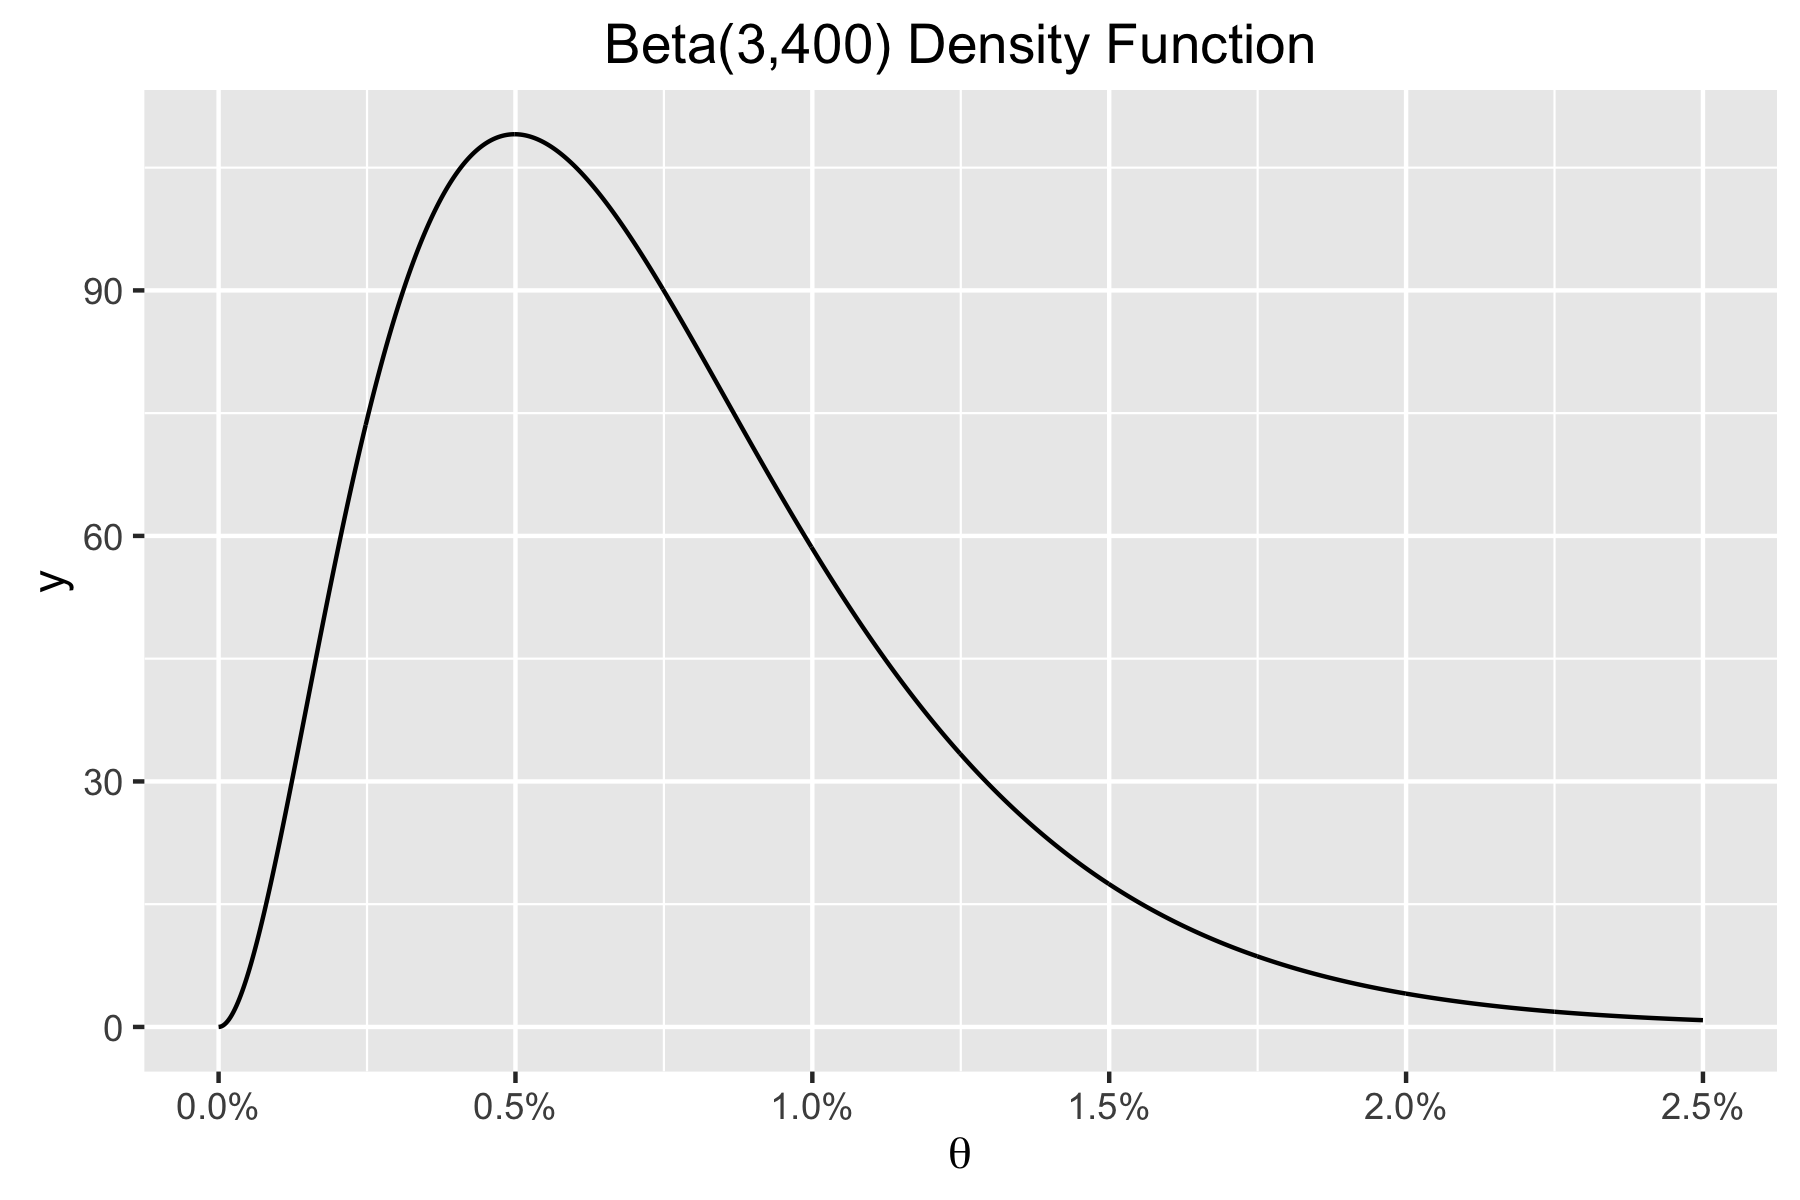
\includegraphics[height=2in]{figures/beta3-400}
\par\end{center}

In this basic Bayesian approach, the parameters $3$ and $400$ would
be chosen by the data scientist based on prior experience, or ``best
guess'', but without looking at the new data. Another approach would
be to use the data to help you choose the parameters $a$ and $b$
in $\mbox{Beta}(a,b)$. This would \textbf{not} be a Bayesian approach,
though it is frequently used in practice. One method in this direction
is called \textbf{empirical Bayes}. Empirical Bayes can be considered
a frequentist approach, in which estimate $a$ and $b$ from the data
$\cd$ using some estimation technique, such as maximum likelihood.
The proper Bayesian approach to this type of thing is called \textbf{hierarchical
Bayes}, in which we put another prior distribution on $a$ and $b$.


\subsubsection*{Mathematical Description}

We'll now give a mathematical description of our model, assuming the
prior parameters $a$ and $b$ are given. Let $n_{1},\ldots,n_{d}$
be the number of impressions we observe for each of the $d$ apps.
In this problem, we will not consider these to be random numbers.
For the $i$th app, let $c_{i}^{1},\ldots,c_{i}^{n_{i}}\in\left\{ 0,1\right\} $
be indicator variables determining whether or not each impression
was clicked. That is, $c_{i}^{j}=\ind{j\mbox{th impression on }i\mbox{th app was clicked}}$.
We can summarize the data on the $i$th app by $\cd_{i}=\left(x_{i},n_{i}\right)$,
where $x_{i}=\sum_{j=1}^{n_{i}}c_{i}^{j}$ is the total number of
impressions that were clicked for app $i$. Let $\theta=(\theta_{1},\ldots,\theta_{d})$,
where $\theta_{i}$ is the CTR for app $i$. 

In our Bayesian approach, we act as though the data were generated
as follows:
\begin{enumerate}
\item Sample $\theta_{1},\ldots,\theta_{d}$ i.i.d. from Beta$(a,b)$. 
\item For each app $i$, sample $c_{i}^{1},\ldots,c_{i}^{n_{i}}$ i.i.d.
from Bernoulli$(\theta_{i})$. 
\end{enumerate}

\subsection{Empirical Bayes for a single app}

We start by working out some details for Bayesian inference for a
single app. That is, suppose we only have the data $\cd_{i}$ from
app $i$, and nothing else. Mathematically, this is exactly the same
setting as the coin tossing setting above, but here we push it further.
\begin{enumerate}
\item Give an expression for $p(\cd_{i}\mid\theta_{i})$, the likelihood
of $\cd_{i}$ given the probability of click $\theta_{i}$, in terms
of $\theta_{i}$, $x_{i}$ and $n_{i}$.\\

\item The probability density for the $\mbox{Beta}(a,b)$ distribution,
evaluated at $\theta_{i}$, is given by
\[
\mbox{Beta}(\theta_{i};a,b)=\frac{1}{B(a,b)}\theta_{i}^{a-1}\left(1-\theta_{i}\right)^{b-1}
\]
where $B(a,b)$ is called the Beta function. Explain why we must have
\[
\int\theta_{i}^{a-1}\left(1-\theta_{i}\right)^{b-1}\,d\theta=B(a,b),
\]
and give the full density function for the prior on $\theta_{i}$,
in terms of $a$, $b$, and the normalization function $B$.\\

\item Give an expression for the posterior distribution $p(\theta_{i}\mid\cd_{i})$.
In this case, include the constant of proportionality. (In other words,
do not use the ``is proportional to'' sign $\propto$ in your final
expression.) {[}Hint: This problem is essentially a repetition of
an earlier problem.{]}\\
 
\item Give a closed form expression for $p(\cd_{i})$, the marginal likelihood
of $\cd_{i}$, in terms of the $a,b,x_{i},$ and $n_{i}$. You may
use the normalization function $B(\cdot,\cdot)$ for convenience,
but you should not have any integrals in your solution. (Hint: $p(\cd_{i})=\int p\left(\cd_{i}\mid\theta_{i}\right)p(\theta_{i})\,d\theta_{i}$,
and the answer will be a ratio of two beta function evaluations.)\\

\item The maximum likelihood estimate for $\theta_{i}$ is $x_{i}/n_{i}$.
Let $p_{\text{MLE}}(\cd_{i})$ be the marginal likelihood of $\cd_{i}$
when we use a prior on $\theta_{i}$ that puts all of its probability
mass at $x_{i}/n_{i}$. Note that 
\begin{eqnarray*}
p_{\text{MLE}}(\cd_{i}) & = & p\left(\cd_{i}\mid\theta_{i}=\frac{x_{i}}{n_{i}}\right)p\left(\theta_{i}=\frac{x_{i}}{n_{i}}\right)\\
 & = & p\left(\cd_{i}\mid\theta_{i}=\frac{x_{i}}{n_{i}}\right).
\end{eqnarray*}
Explain why, or prove, that $p_{\text{MLE}}(\cd_{i})$ is larger than
$p(\cd_{i})$ for any other prior we might put on $\theta_{i}$. If
it's too hard to reason about all possible priors, it's fine to just
consider all Beta priors. {[}Hint: This does not require much or any
calculation. It may help to think about the integral $p(\cd_{i})=\int p\left(\cd_{i}\mid\theta_{i}\right)p(\theta_{i})\,d\theta_{i}$
as a weighted average of $p(\cd_{i}\mid\theta_{i})$ for different
values of $\theta_{i}$, where the weights are $p(\theta_{i})$.{]}\\

\item One approach to getting an \textbf{empirical Bayes} estimate of the
parameters $a$ and $b$ is to use maximum likelihood. Such an empirical
Bayes estimate is often called an \textbf{ML-2} estimate, since it's
maximum likelihood, but at a higher level in the Bayesian hierarchy.
To emphasize the dependence of the likelihood of $\cd_{i}$ on the
parameters $a$ and $b$, we'll now write it as $p(\cd_{i}\mid a,b)$\footnote{Note that this is a slight (though common) abuse of notation, because
$a$ and $b$ are not random variables in this setting. It might be
more appropriate to write this as $p(\cd_{i};a,b)$ or $p_{a,b}(\cd_{i})$.
But this isn't very common.}. The empirical Bayes estimates for $a$ and $b$ are given by
\[
(\hat{a},\hat{b})=\argmax_{\left(a,b\right)\in\reals^{>0}\times\reals^{>0}}p(\cd_{i}\mid a,b).
\]
To make things concrete, suppose we observed $x_{i}=3$ clicks out
of $n_{i}=500$ impressions. A plot of $p(\cd_{i}\mid a,b)$ as a
function of $a$ and $b$ is given in Figure \ref{fig:single-app-contour-plot}.
\begin{figure}
\centering{}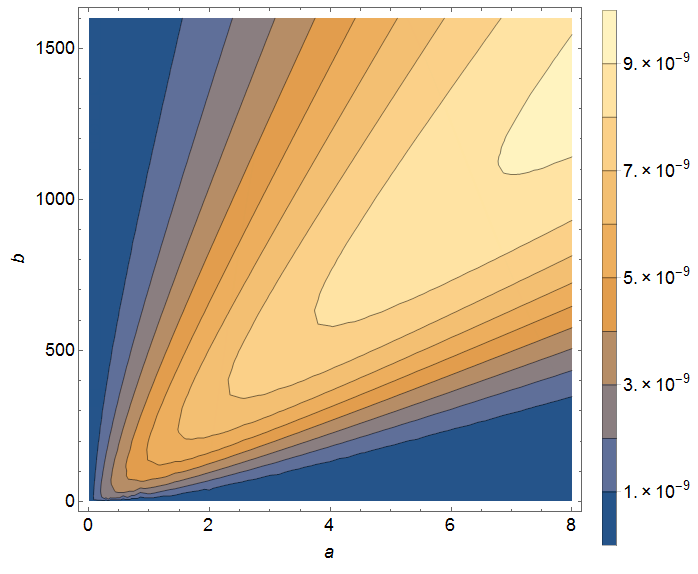
\includegraphics[height=2.5in]{figures/single-app-marginal-lik-contour-plot}\caption{\label{fig:single-app-contour-plot}A plot of $p(\protect\cd_{i}\mid a,b)$
as a function of $a$ and $b$. }
\end{figure}
It appears from this plot that the likelihood will keep increasing
as $a$ and $b$ increase, at least if $a$ and $b$ maintain a particular
ratio. Indeed, this likelihood function never attains its maximum,
so we cannot use ML-2 here. Explain what's happening to the prior
as we continue to increase the likelihood. {[}Hint: It is a property
of the Beta distribution (not difficult to see), that for any $\theta\in\left(0,1\right)$,
there is a Beta distribution with expected value $\theta$ and variance
less than $\eps$, for any $\eps>0$. What's going in here is similar
to what happens when you attempt to fit a gaussian distribution $\cn(\mu,\sigma^{2})$
to a single data point using maximum likelihood.{]}\\

\end{enumerate}

\subsection{Empirical Bayes Using All App Data}

In the previous section, we considered working with data from a single
app. With a fixed prior, such as Beta(3,400), our Bayesian estimates
for $\theta_{i}$ seem more reasonable (to me, the person who chose
the prior) than the MLE when our sample size $n_{i}$ is small. The
fact that these estimates seem reasonable is an immediate consequence
of the fact that I chose the prior to give high probability to estimates
that seem reasonable to me, before ever seeing the data. Our attempt
to use empirical Bayes (ML-2) to choose the prior in a data-driven
way was not successful. With only a single app, we were essentially
overfitting the prior to the data we have. In this section, we'll
consider using the data from all the apps, in which case empirical
Bayes makes more sense.
\begin{enumerate}
\item Let $\cd=\left(\cd_{1},\ldots,\cd_{d}\right)$ be the data from all
the apps. Give an expression for $p(\cd\mid a,b)$, the \textbf{marginal
likelihood} of $\cd$. Expression should be in terms of $a,b,x_{i},n_{i}$
for $i=1,\ldots,d$. (Hint: This problem should be easy, based on
a problem from the previous section.) \end{enumerate}

\end{document}
